\documentclass{article}

\usepackage{graphicx}
\usepackage{multirow}

\title{Note: Regularization}
\author{Sun Zhao}

\begin{document}
\maketitle
\newpage

\section{Over-fitting}
Over-fitting problem occurs when the learned hypothesis fits the training data set very well, but fails to generalize to new examples. It is mainly coursed by the trained model is excessively complex, such as having too many parameters relative to the number of observations. Fig. \ref{over-fitting_linear_regression_example} shows three linear regression hypothesises for the house prices predicting problem. The hypothesis shown in Fig. \ref{over-fitting_linear_regression_example}A is called "under-fitting" which means it is quite bias from the right one. Fig. \ref{over-fitting_linear_regression_example}C is an example of over-fitting which has high variance. Though it predicts the prices perfectly for every examples in training data, it can not be generalized to new input. Moreover, Fig. \ref{over-fitting_logistic_regression_example} shows "under-fitting", "right one", "over-fitting" logistic regression hypothesis separately.

\begin{figure}[ht]
  \centering
  % Requires \usepackage{graphicx}
  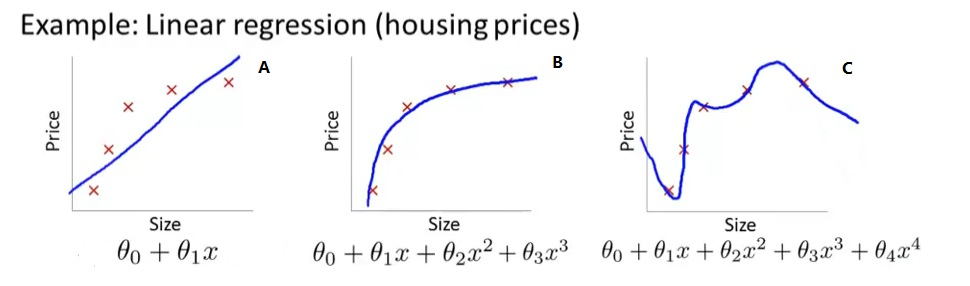
\includegraphics[width=10cm]{Figure1.jpg}\\
  \caption{}\label{over-fitting_linear_regression_example}
\end{figure}

\begin{figure}[ht]
  \centering
  % Requires \usepackage{graphicx}
  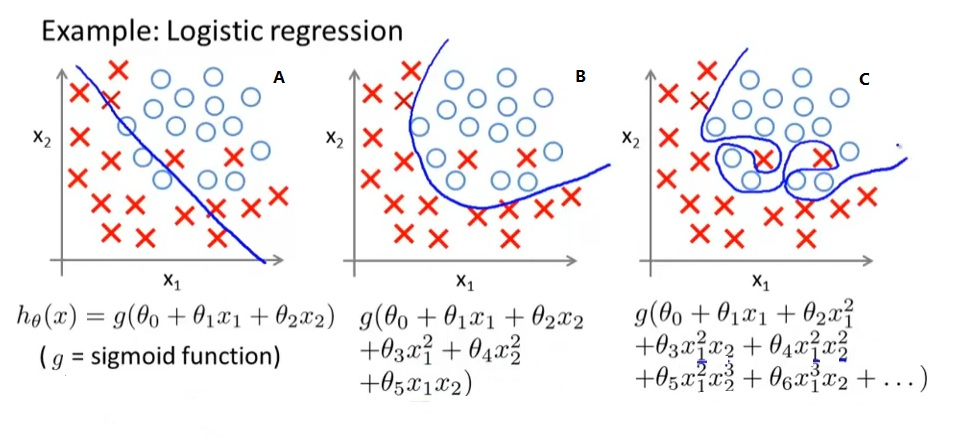
\includegraphics[width=10cm]{Figure2.jpg}\\
  \caption{}\label{over-fitting_logistic_regression_example}
\end{figure}

\section{Regularized Cost Function}
The intuition of regularization is to penalize large parameters of $\theta$ and keep the hypothesis simple. In Fig. \ref{over-fitting_linear_regression_example}C, if we can penalize $\theta_{4}$ and shrink it to zero, the hypothesis will much closer to the "right" one. Regularization adds a term of $\frac{\lambda}{2m} \sum_{j=1}^{n}\theta_{j}$ to the regression cost function. So, the new cost function is as (\ref{regular_cost_function}).
\begin{equation}\label{regular_cost_function}
J^{'}(\theta) = J(\theta) + \frac{\lambda}{2m} \sum_{j=1}^{n}\theta_{j}
\end{equation}
The larger value of $\theta_{j}$, the larger cost of the corresponding hypothesis, hence the gradient descent algorithm will penalize large $\theta_{j}$.  

\section{Regularized Gradient Descent}
\end{document}
